\section{Build-time}

\subsection*{Purpose}
To compare the time taken for the creation of each sketch under different types of graph streams.

\subsection*{Results}

\begin{figure}[H]
    \centering 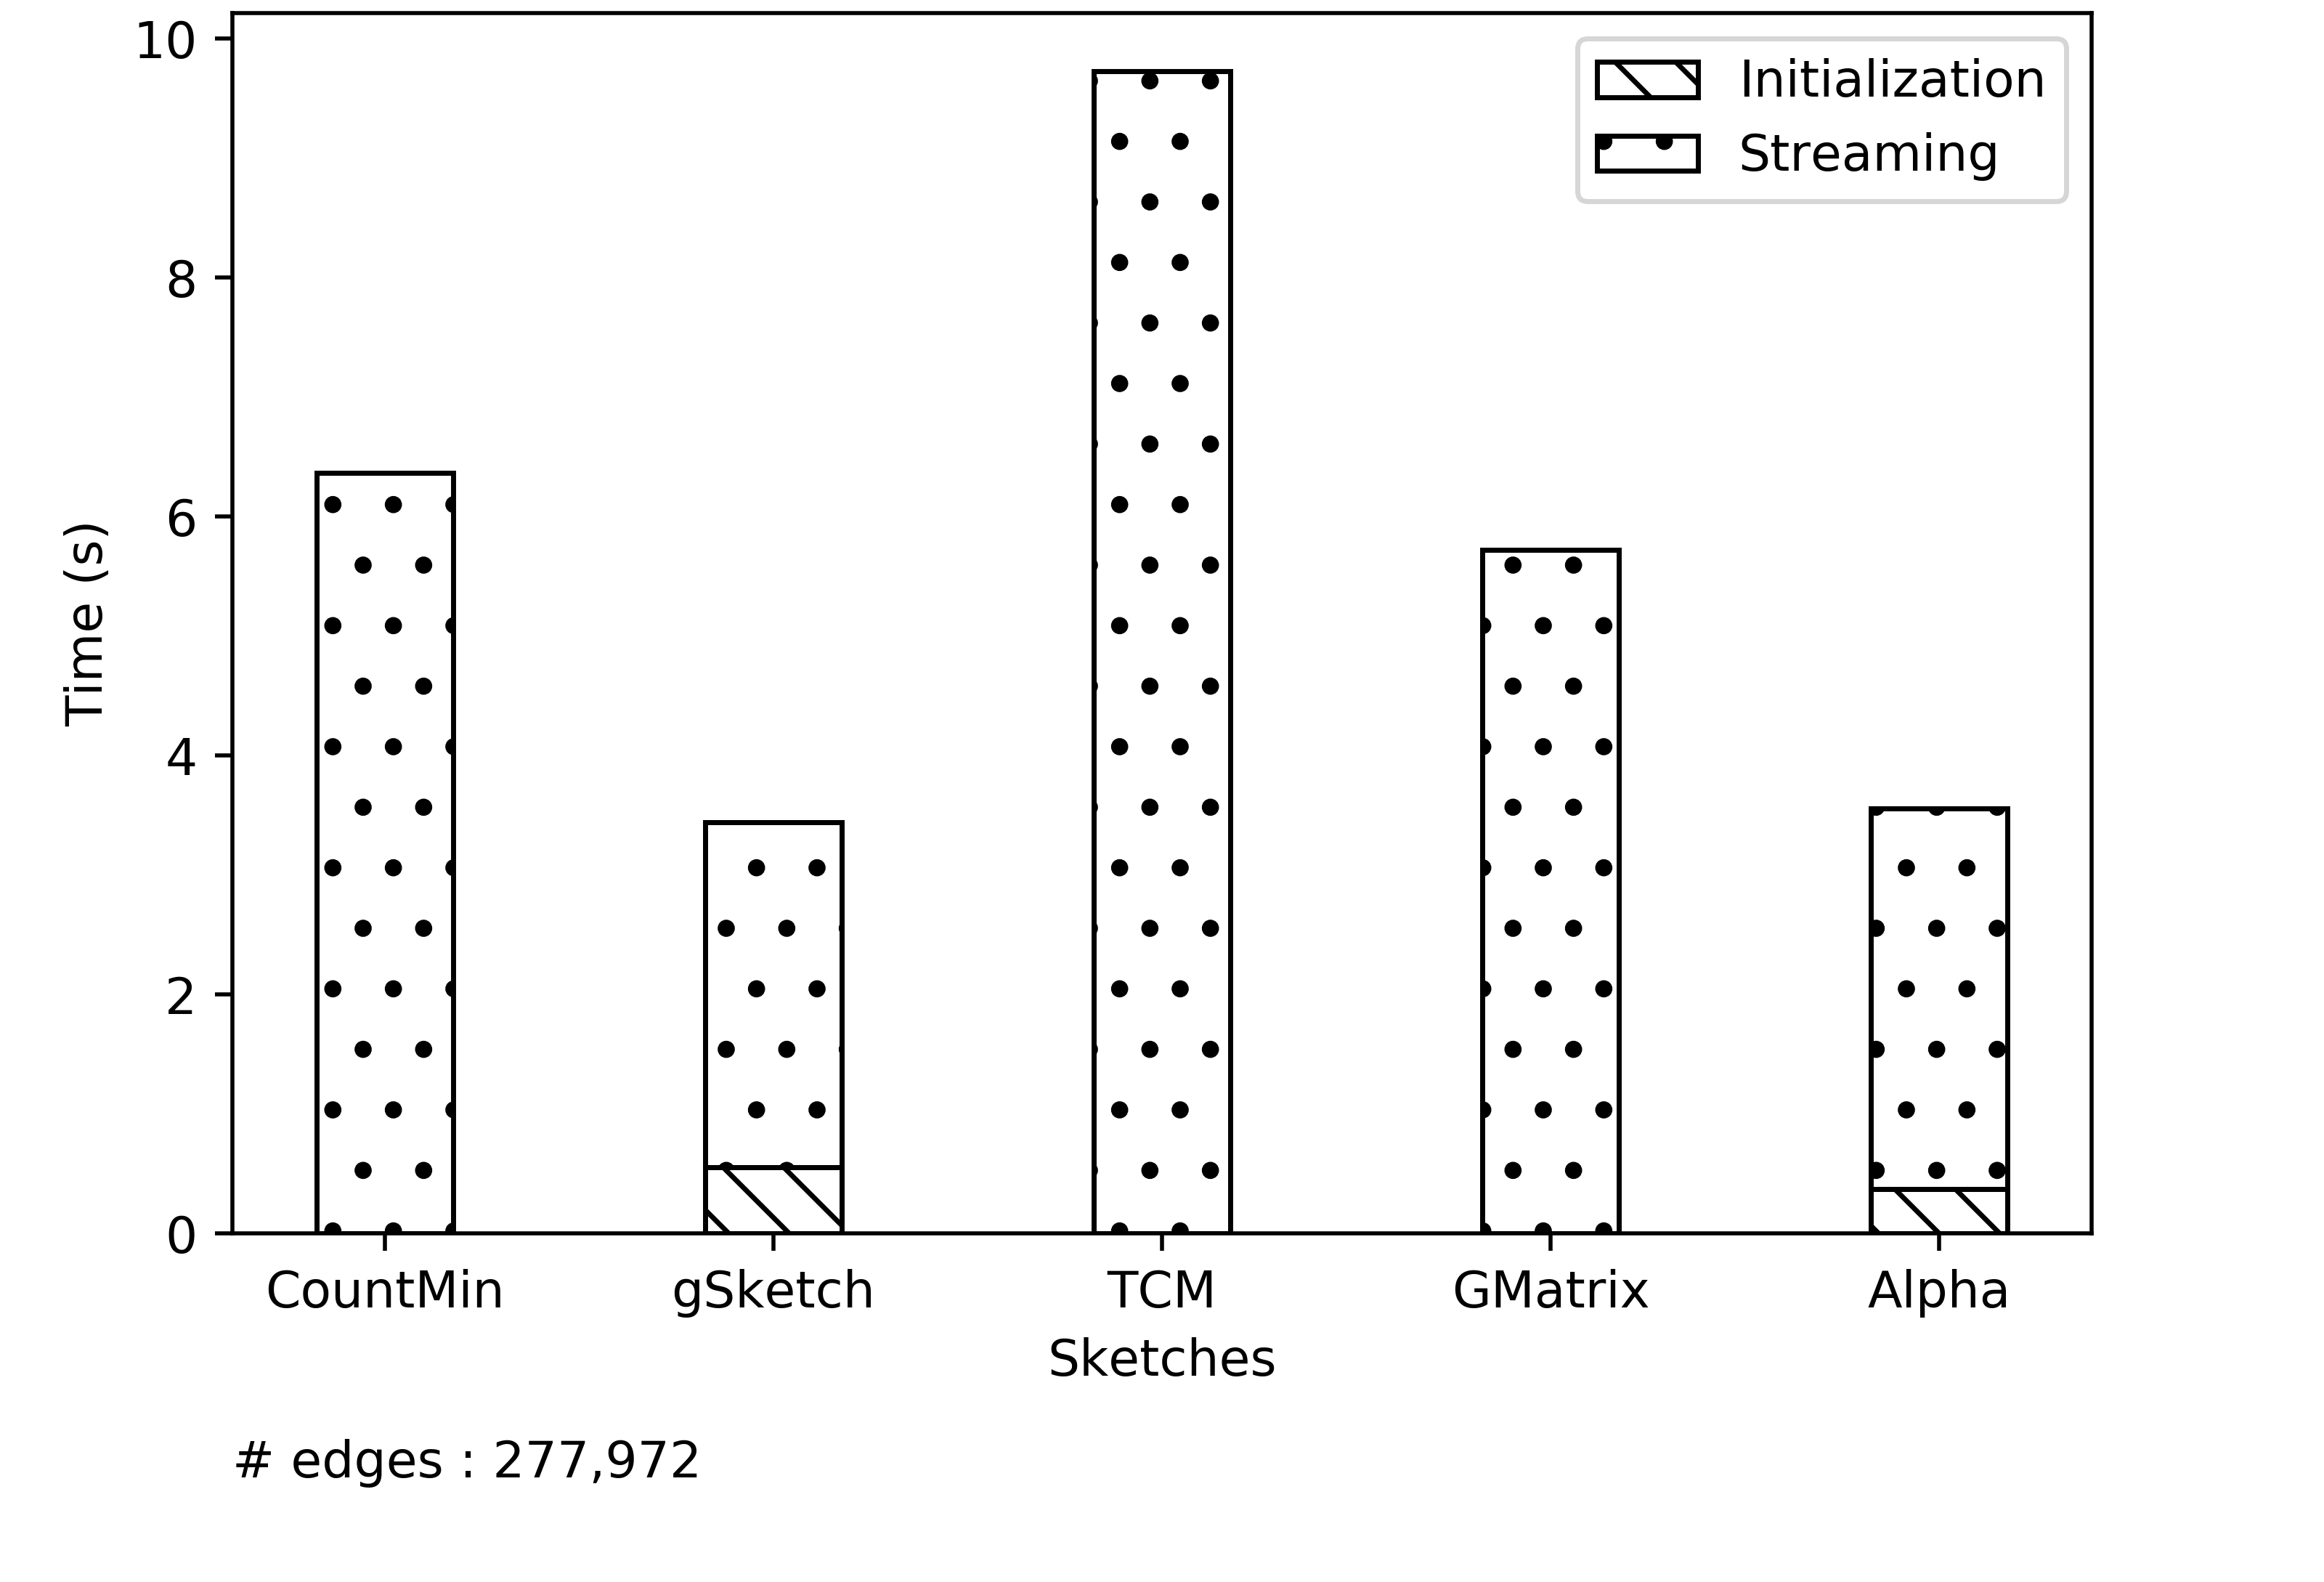
\includegraphics[width=0.85\textwidth]{results/buildtime/unicorn-wget-buildtime_1024}
    \vspace{-0.5cm}
    \caption{Build-time for unicorn-wget dataset}
    \label{fig:unicorn-wget-buildtime_1024}
\end{figure}

\begin{figure}[H]
    \centering 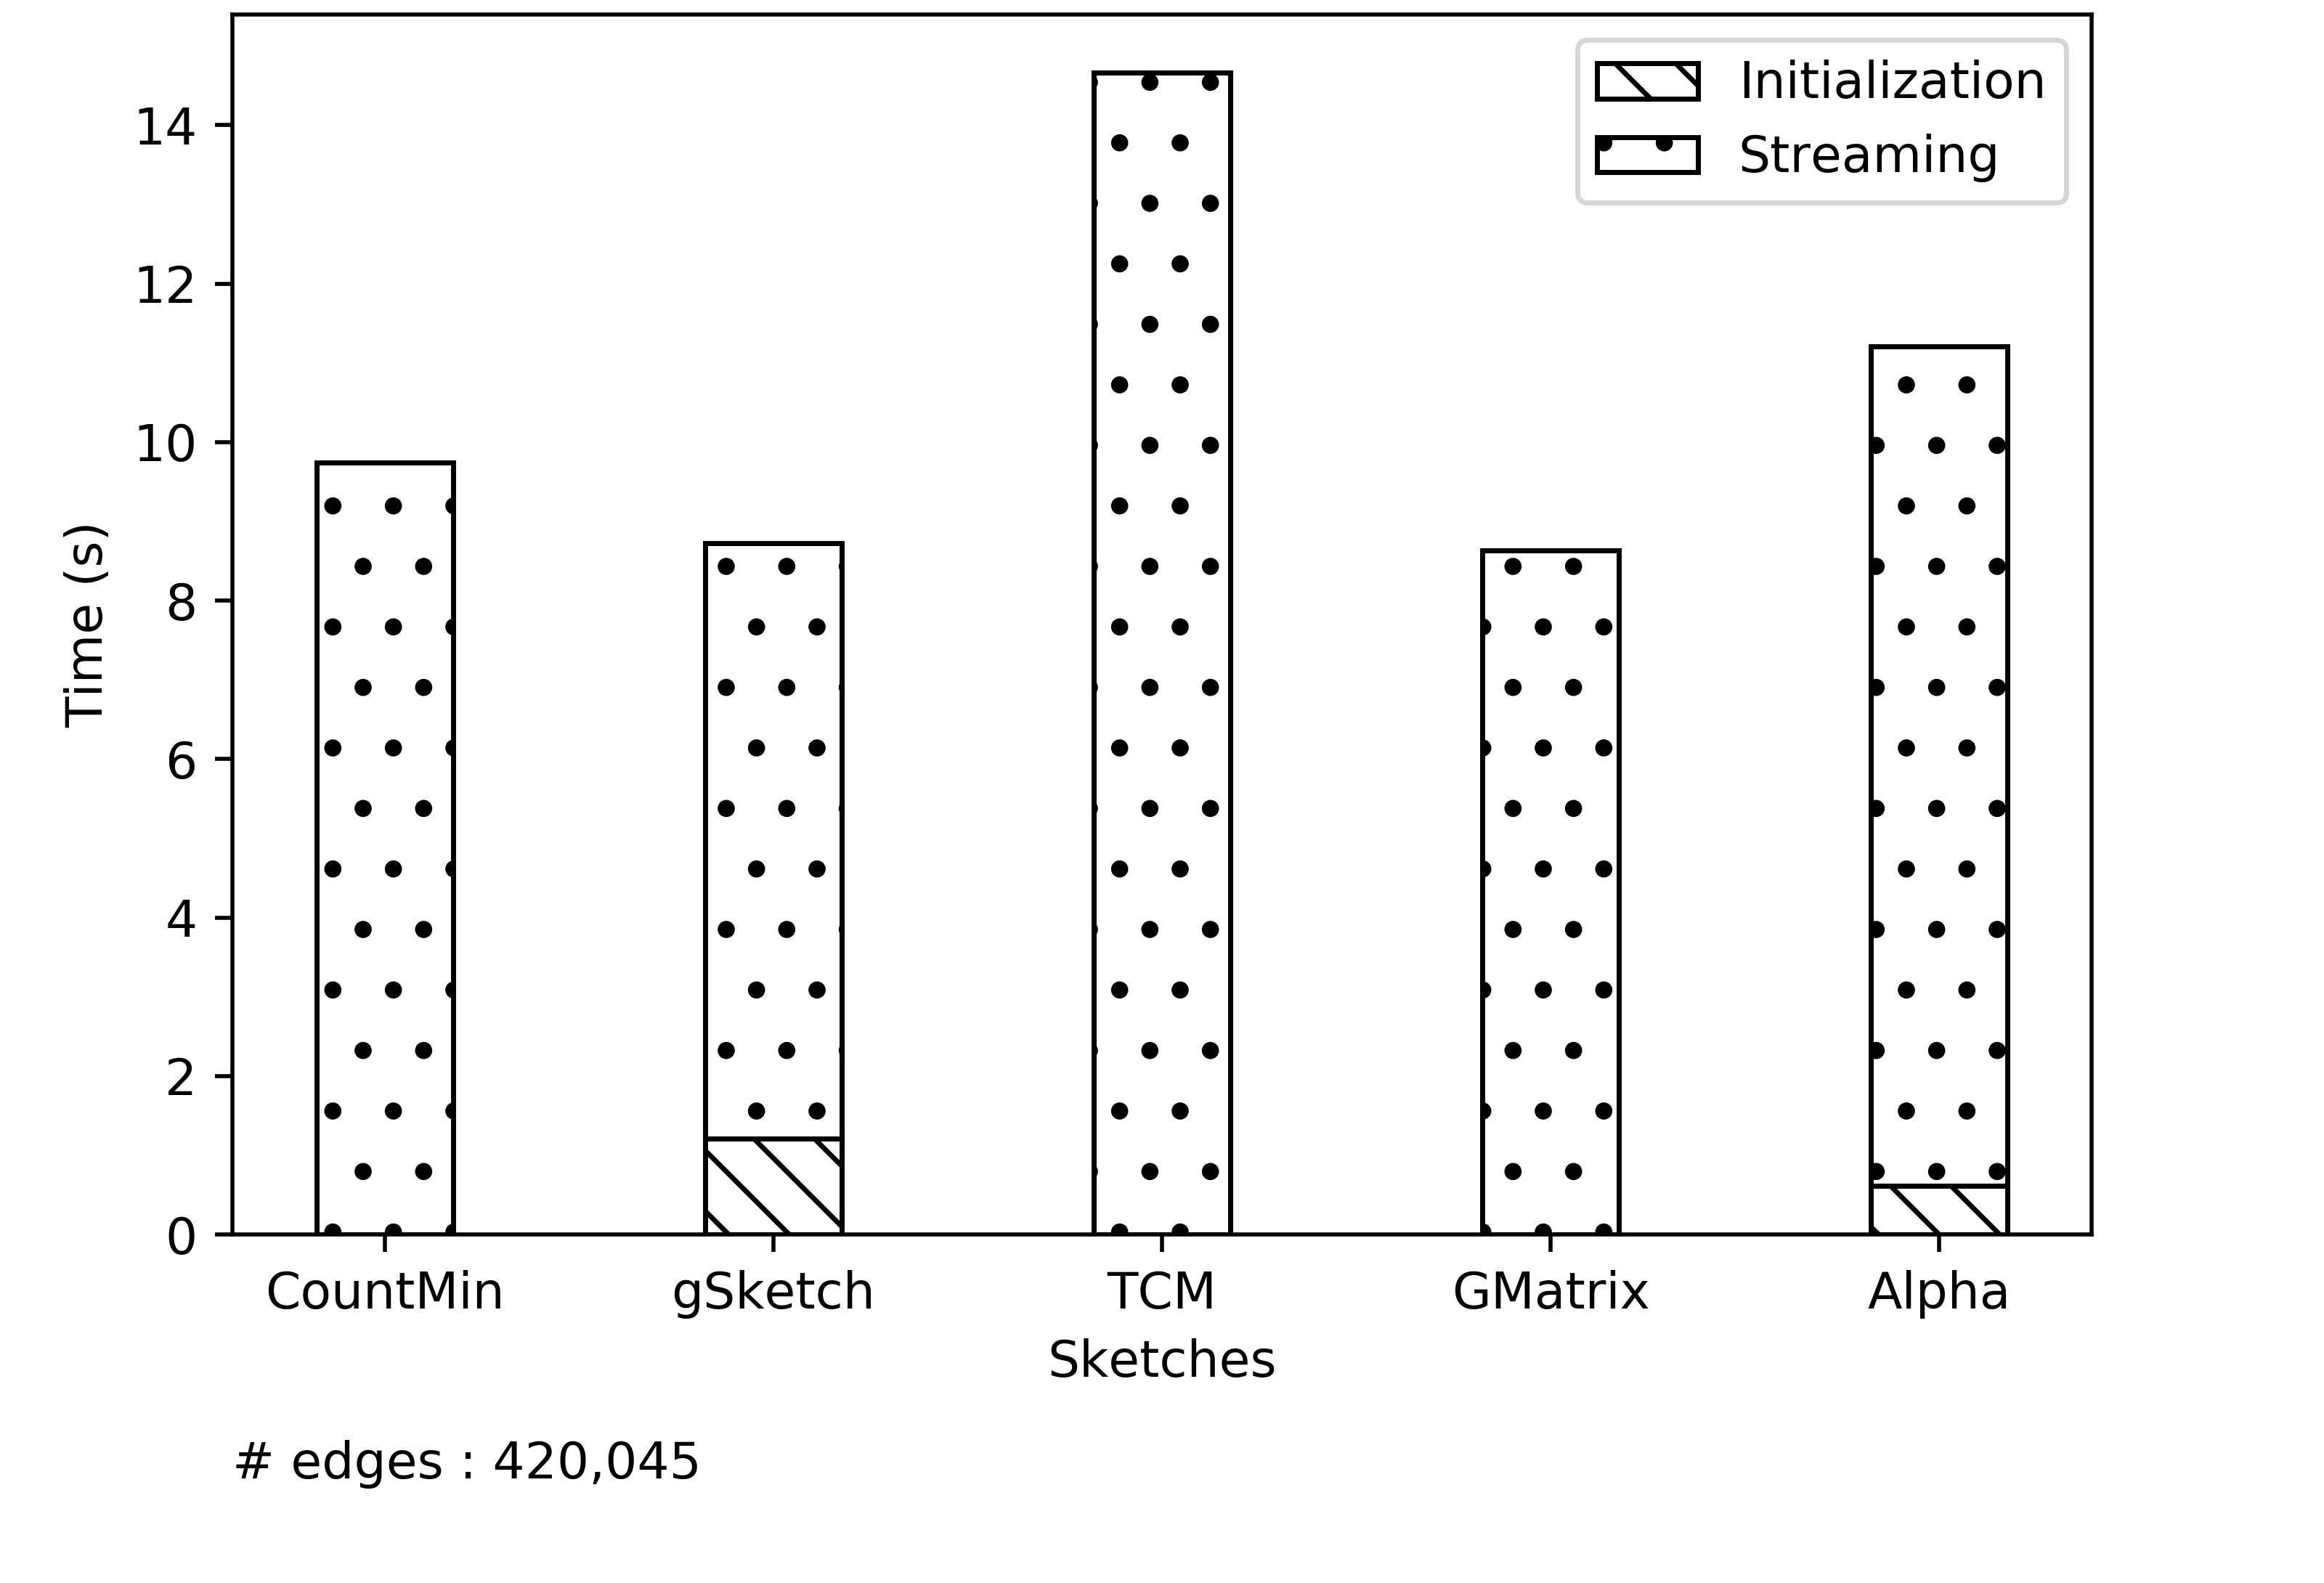
\includegraphics[width=0.85\textwidth]{results/buildtime/email-EuAll-buildtime_1024}
    \vspace{-0.5cm}
    \caption{Build-time for email-EuAll dataset}
    \label{fig:email-EuAll-buildtime_1024}
\end{figure}

\begin{figure}[H]
    \centering 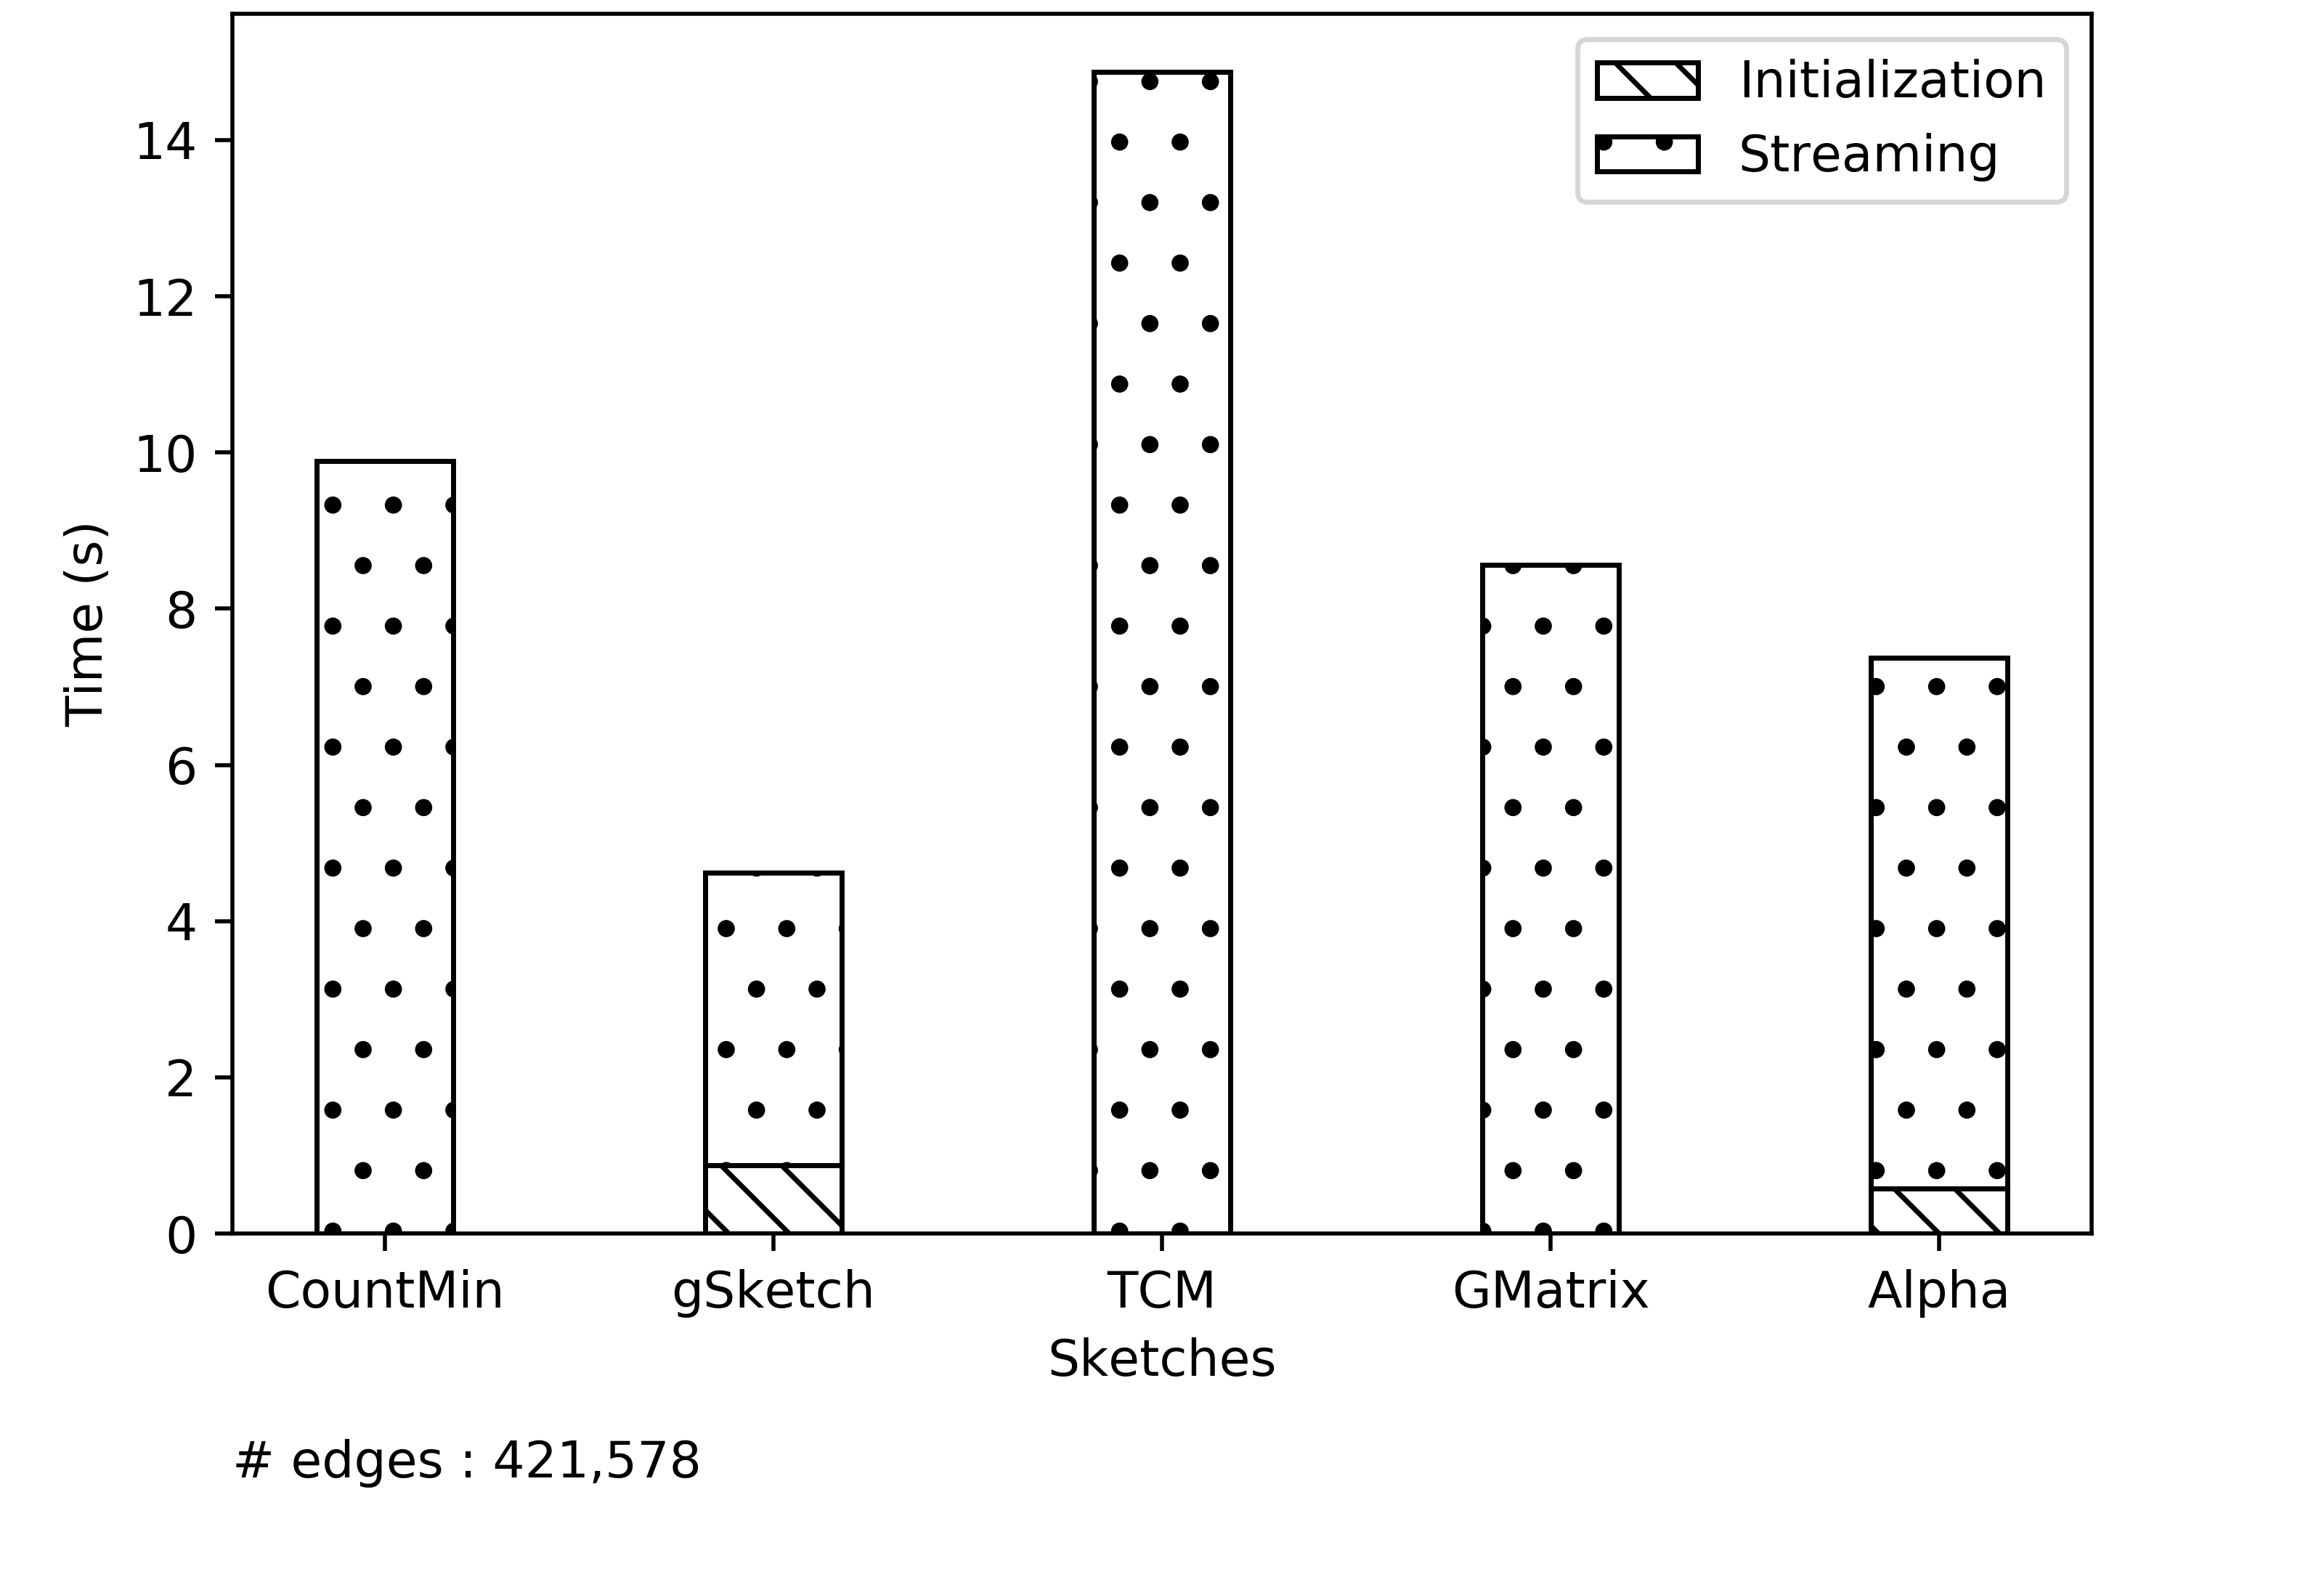
\includegraphics[width=0.85\textwidth]{results/buildtime/cit-HepPh-buildtime_1024}
    \vspace{-0.5cm}
    \caption{Build-time for cit-HepPh dataset}
    \label{fig:cit-HepPh-buildtime_1024}
\end{figure}

\begin{figure}[H]
    \centering 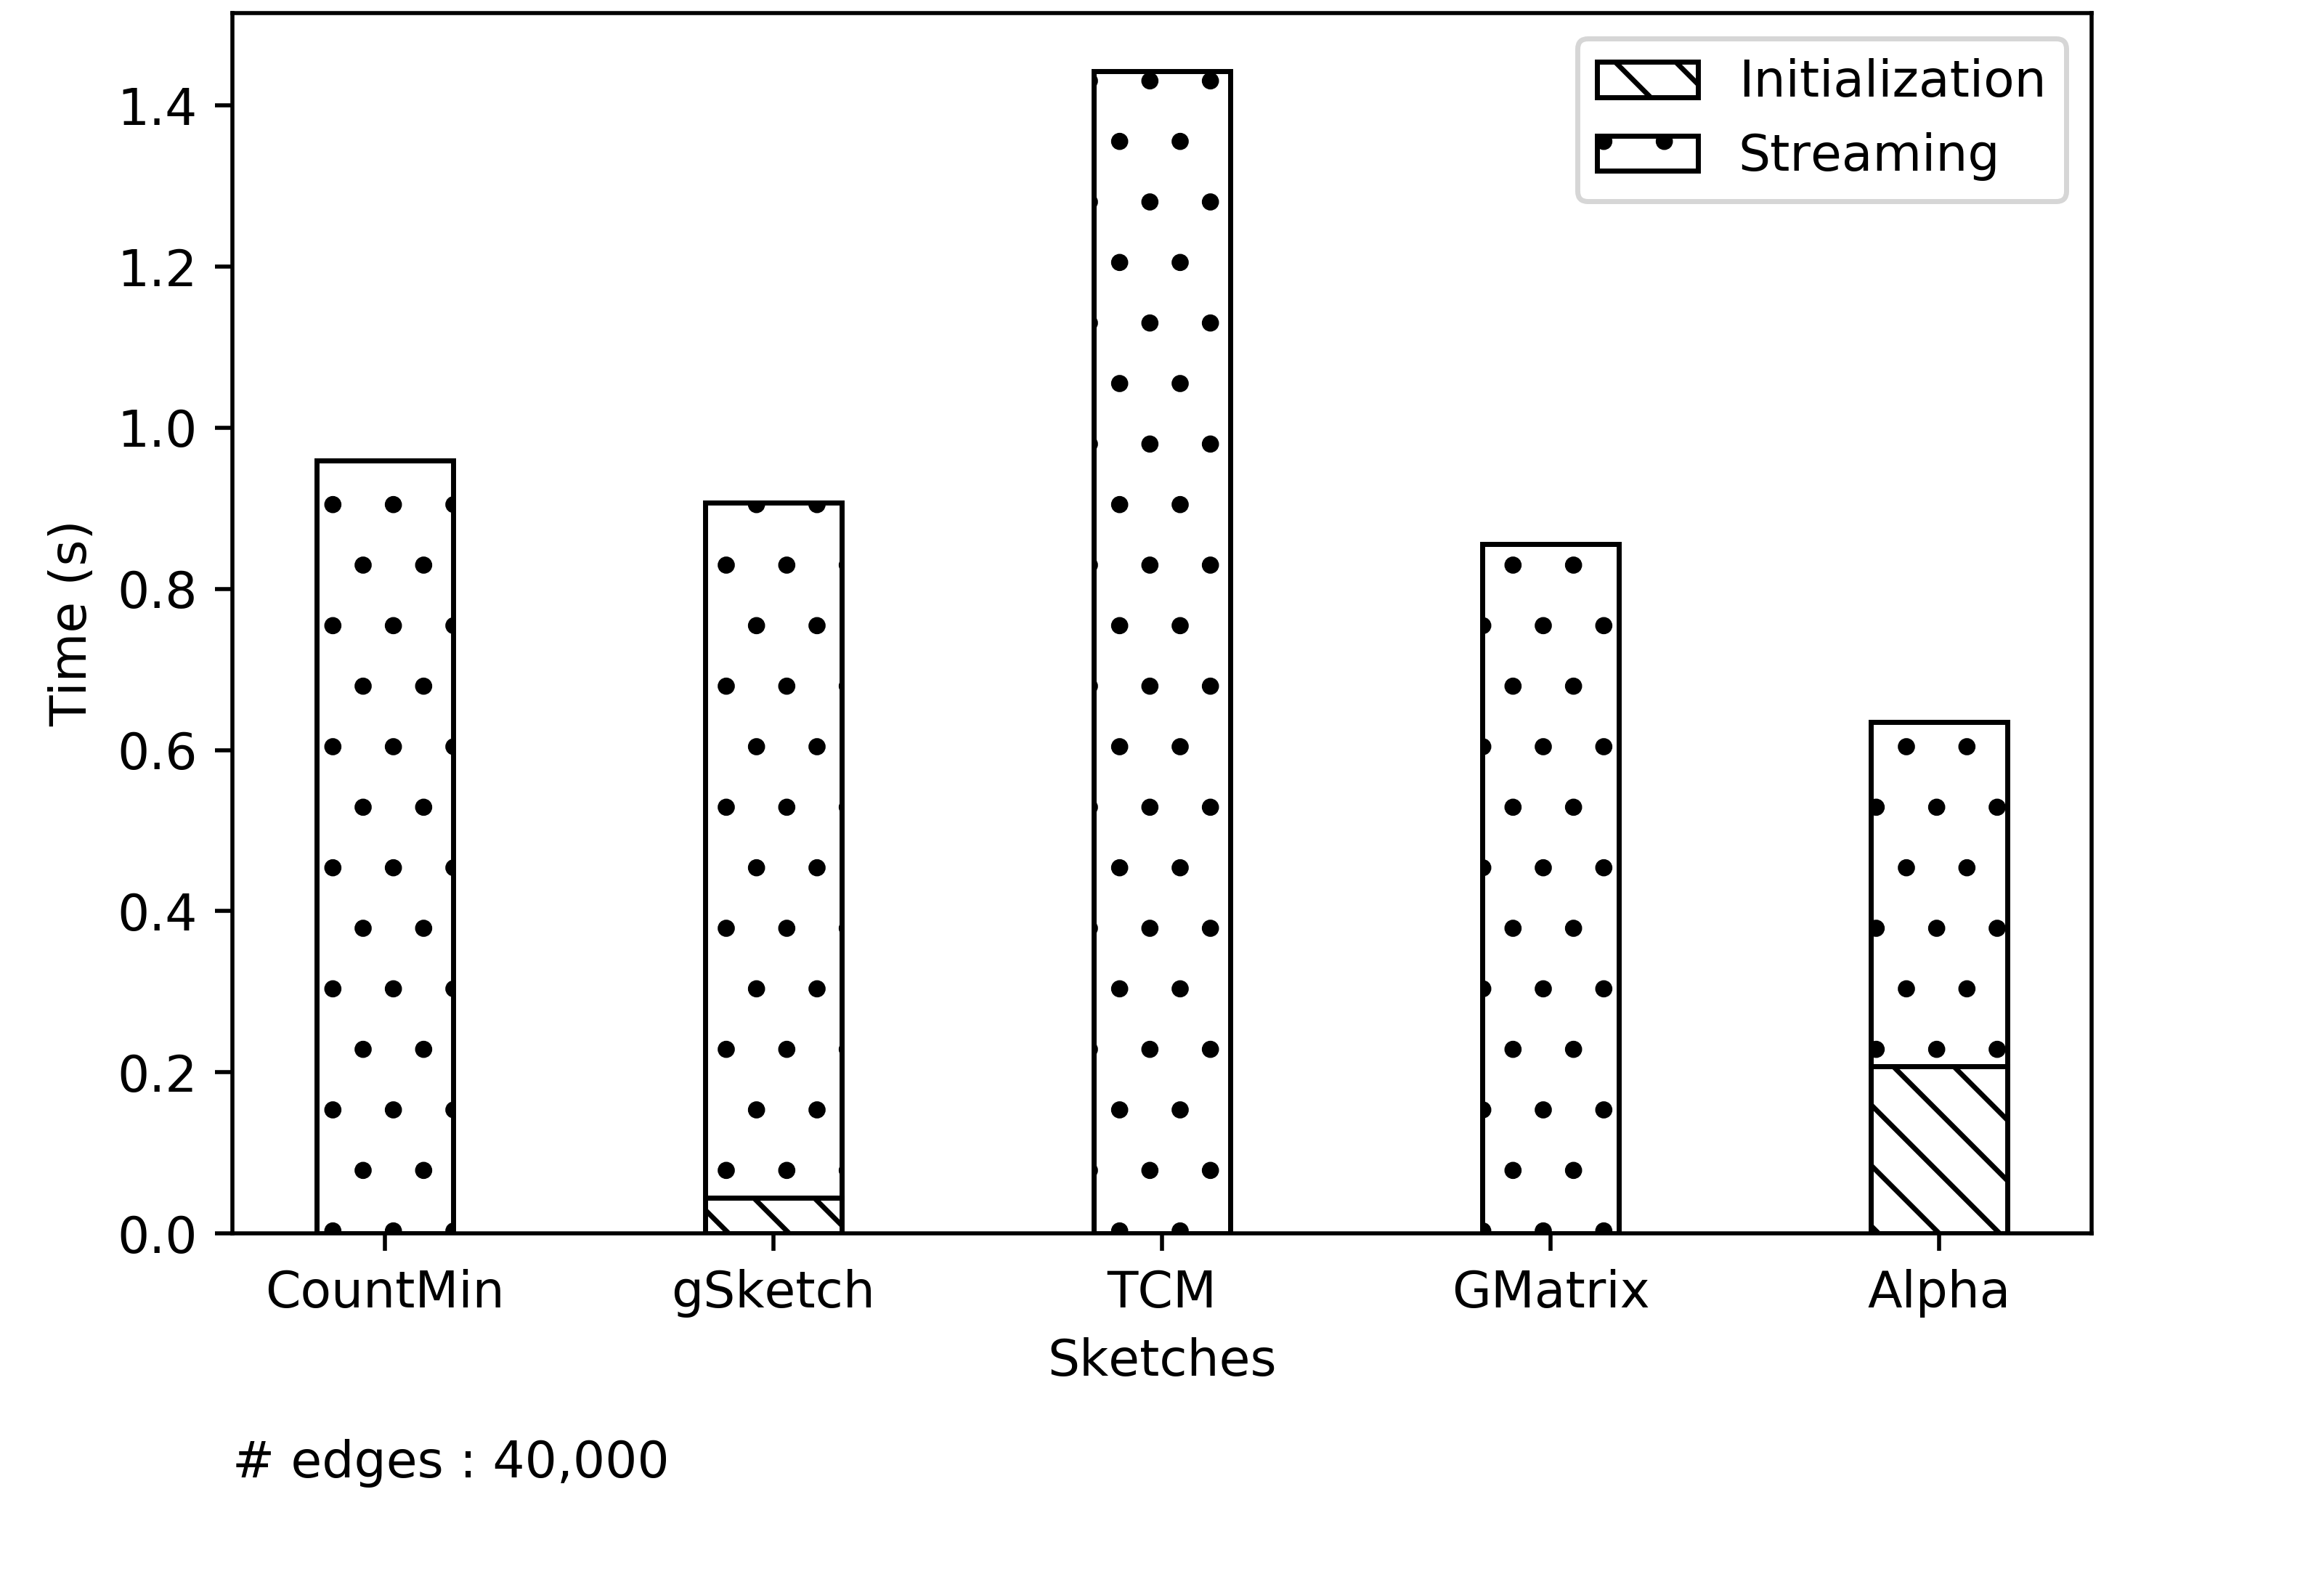
\includegraphics[width=0.85\textwidth]{results/buildtime/gen-scale-free-buildtime_1024}
    \vspace{-0.5cm}
    \caption{Build-time for gen-scale-free dataset}
    \label{fig:gen-scale-free-buildtime_1024}
\end{figure}

\begin{figure}[H]
    \centering 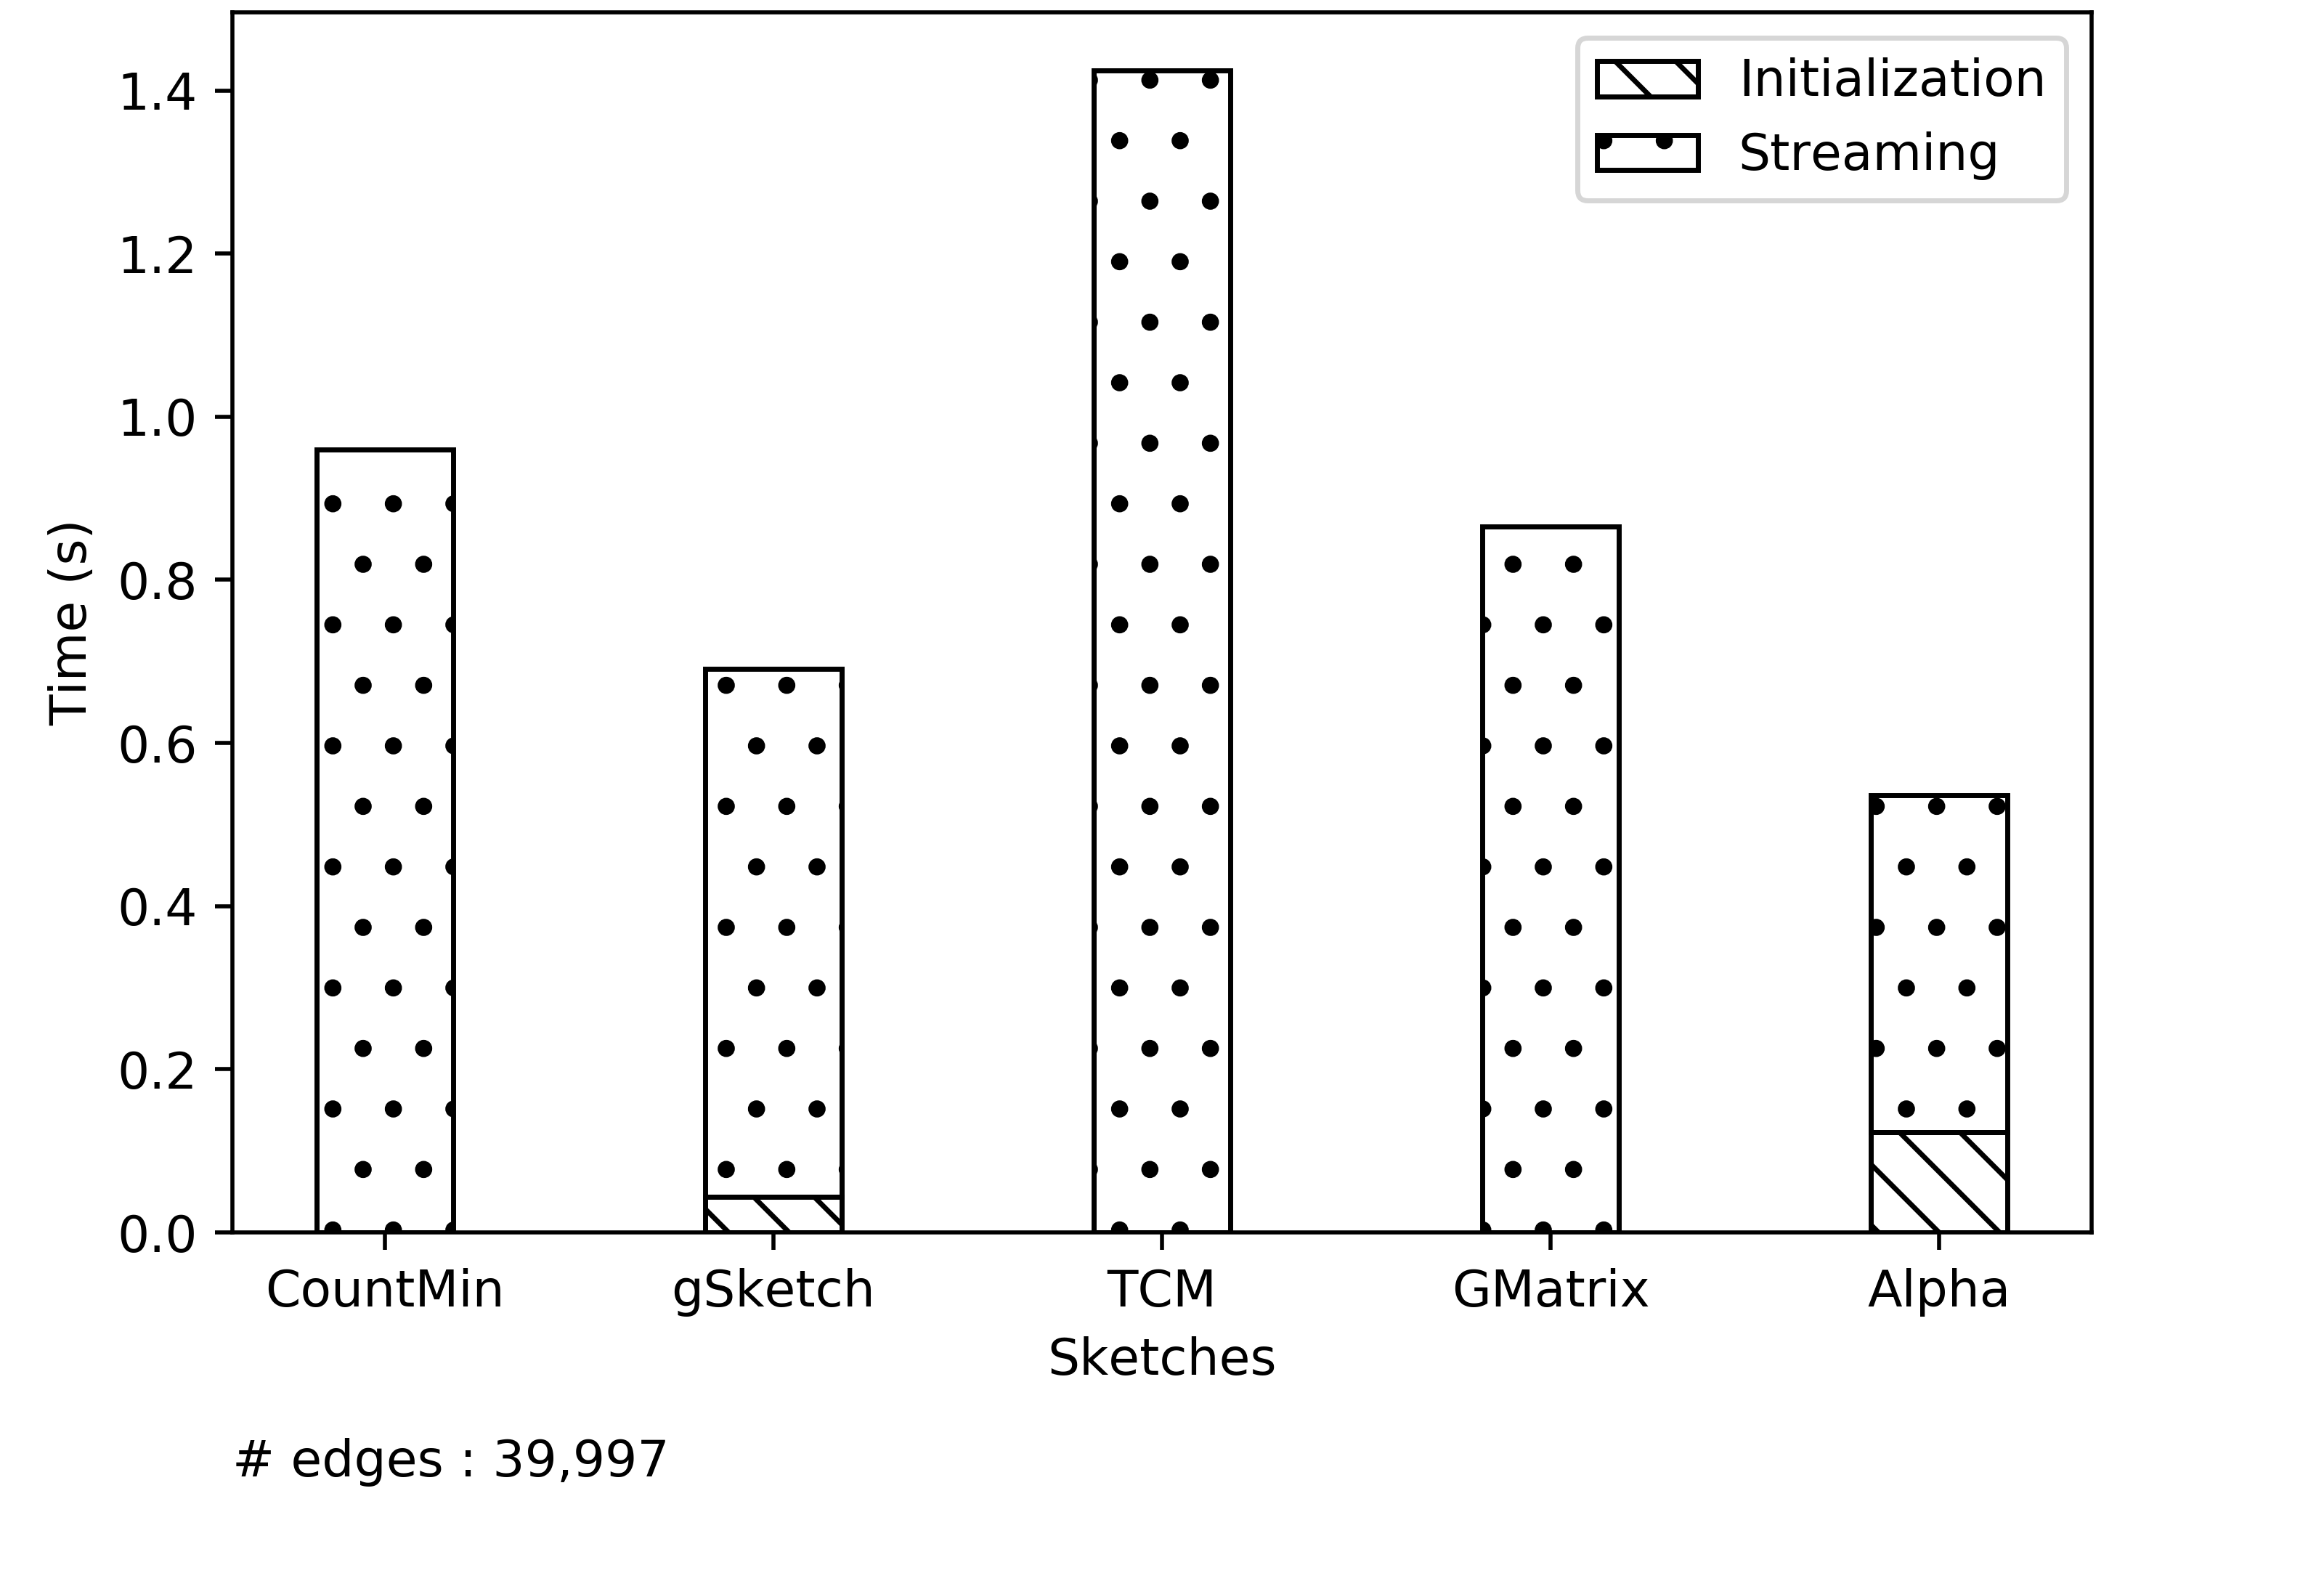
\includegraphics[width=0.85\textwidth]{results/buildtime/gen-small-world-buildtime_1024}
    \vspace{-0.5cm}
    \caption{Build-time for gen-small-world dataset}
    \label{fig:gen-small-world-buildtime_1024}
\end{figure}

\subsection*{Observations and inferences}

\paragraph{}
Both the gSketch and Alpha has been initialized with a sample of 10,000 edges from the original stream. Thus the gSketch and Alpha have comparable initialization times. The other sketches do not have an initialization time cost as they don't possess initialization stages. All the sketches were created with 1 MB memory allocation.

\paragraph{}
In the results for the datasets, unicorn-wget in \autoref{fig:unicorn-wget-buildtime_1024}, cit-HepPh in \autoref{fig:cit-HepPh-buildtime_1024}, gen-scale-free in \autoref{fig:gen-scale-free-buildtime_1024} and gen-small-world in \autoref{fig:gen-small-world-buildtime_1024}; Alpha has taken a significantly lower time for the streaming than all the other sketches except for gSketch.

\paragraph{}
Sketch creation and the streaming time of Alpha is significantly better than the CountMin, TCM and GMatrix for 4/5 datasets that were tested. Only gSketch has performed slightly better than Alpha in this regard. However this can be dismissed as gSketch is a only a frequency approximation sketch. Therefor we are able to conclude that Alpha is generally faster than the existing sketching techniques in creation of the summarized sketch.